% vim: set spell spelllang=es syntax=tex :

\section{Descripción del sistema}

Para aumentar el throughput del sistema se pueden aplicar cuatro enfoques distintos:

\begin{itemize}

	\item 	Dado que en un vídeo ya decodificado el procesamiento de cada
		cuadro es independiente del procesamiento de los demás, y dada
		la disponibilidad de recursos de computo, se pueden procesar
		múltiples cuadros al mismo tiempo sin que esto genere
		diferencias en la información obtenida (salvo por el orden).
		Esto permitiría aumentar la cantidad de cuadros por segundo
		obtenidos, aunque el tiempo de procesamiento de cada uno se
		mantenga igual.

	\item	Para realizar la búsqueda de los objetos, el cuadro puede ser
		dividido. Esto permitirá realizar la búsqueda en cada zona en
		paralelo. Para el correcto funcionamiento, las zonas deberán
		tener partes en común que dependerán del tamaño de los objetos,
		ya que no debe suceder que un objeto no aparezca completo en
		ninguna de las zonas. Esto permitiría reducir el tiempo de
		procesamiento de cada cuadro, ademas de que se puede sacar
		provecho de una mayor localidad espacial.

	\item	Ya que la búsqueda de cada tipo de objetos es independiente de
		la búsqueda de los demás tipos, se pueden realizar múltiples
		búsquedas en paralelo sobre el mismo cuadro por cada tipo de
		objeto.

	\item	Se puede resolver el problema optimizando cada uno de los
		plugins del framework, esperando de esta manera que el tiempo de
		procesamiento de cada cuadro se reduzca lo suficiente como para
		que el sistema pueda procesar la mayoría de los cuadros a
		tiempo.

\end{itemize}

Lamentablemente este último enfoque dificulta su uso como herramienta didáctica,
ya que cada plugin que se agregue o modifique deberá ser optimizado. El primer y
segundo enfoque permiten agregar y modificar los plugins sin mayores
dificultades, y en el caso en el cual un plugin no cumpla con las condiciones
que permitan aplicar alguno de los enfoques, se puede limitar el paralelismo ya
sea no dividiendo el cuadro o procesando solo uno por vez.

Si bien el tercer enfoque también permitiría agregar o modificar los plugins
fácilmente, en las pruebas que se realizaron se comprobó que realizar las
búsquedas por cada tipo de objeto en paralelo sobre cada fragmento tenia un
efecto adverso. Por este motivo, el tercer enfoque no fue aplicado sobre el
producto final, y no sera incluido en las explicaciones siguientes. Los detalles
de los resultados que llevaron a tomar esta decisión serán detallados mas
adelante en la sección de resultados.

\subsection{Tareas del sistema}

El sistema ejecuta tareas estáticas y tareas dinámicas. Las tareas estáticas son
aquellas que permanecen en ejecución desde el inicio del programa hasta su
finalización. Las tareas dinámicas son creadas para procesar un cuadro o
fragmento específico y una vez que terminan de procesar el cuadro o fragmento
finalizan. Como las tareas dinámicas son aquellas que realizan el procesamiento
para la búsqueda de los objetos, las llamamos "tareas de búsqueda".

Según su funcionalidad, las tareas son clasificadas en cuatro tipos:

\begin{description}

	\item[Generación de cuadros:] Es la tarea encargada de la generación o
		captura de los cuadros y colocarlos en la cola de cuadros a
		procesar. Esta es una tarea estática, y sólo hay una en el
		sistema.

	\item[Generación de tareas de fragmentación de cuadro:] Esta tarea crea
		una tarea de fragmentación de cuadro para cada cuadro en la
		cola. Solo toma un cuadro de la cola si hay hilos de ejecución
		para tareas de búsqueda libres. Ésta es una tarea estática, y
		solo hay una en el sistema.

	\item[Fragmentación de cuadro:] Cada tarea de este tipo divide su cuadro
		en una cantidad predefinida de fragmentos de igual (o similar)
		tamaño. Luego, por cada fragmento, se crea una tarea de
		procesamiento de fragmento. Estas son tareas de búsqueda, y
		puede haber múltiples en el sistema.

	\item[Procesamiento de fragmento:] Cada una de estas tareas toma su
		fragmento asociado y lo procesa utilizando cada una de las pilas
		de plugins. Estas son tareas de búsqueda, y puede haber
		múltiples en el sistema.

\end{description}

\begin{figure}[!h]

	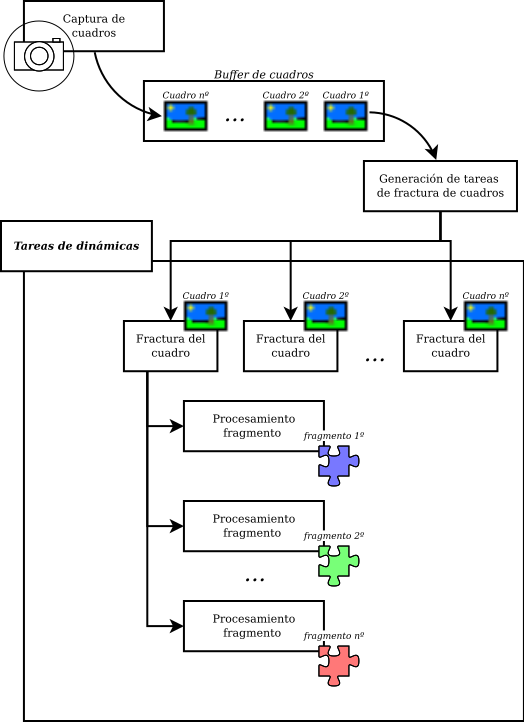
\includegraphics[width=\textwidth]{img/framework.pdf}

	\caption{Tareas principales del framework.}

	\label{tareasFramework}

\end{figure}

Cada una de las dos tareas estáticas tiene un hilo de ejecución asignado. Las
tareas de búsqueda son ejecutadas por un conjunto de $N$ hilos de
ejecución\footnote{$N$ es un parámetro de entrada del programa.}. Cuando un hilo
de ejecución (del conjunto) está libre, toma una nueva tarea de búsqueda para
ejecutar. Como estos hilos de ejecución son los que ejecutan las tareas de
búsqueda, nos referiremos a ellos como "hilos de búsqueda". En la figura
\ref{tareasFramework} se muestran un diagrama de las tareas del framework, y en
la figura \ref{hilosFramework} se muestra como las tareas son asignadas a los
hilos de ejecución.

La cantidad de hilos de ejecución del sistema es igual a la cantidad de hilos de
búsqueda mas los dos hilos para tareas estáticas (generación de cuadros y
generación de tareas de fragmentación de cuadro). Por esto la cantidad de
unidades de procesamiento aprovechables esta principalmente determinado por la
cantidad de hilos de búsqueda.

\begin{figure}[!h]

	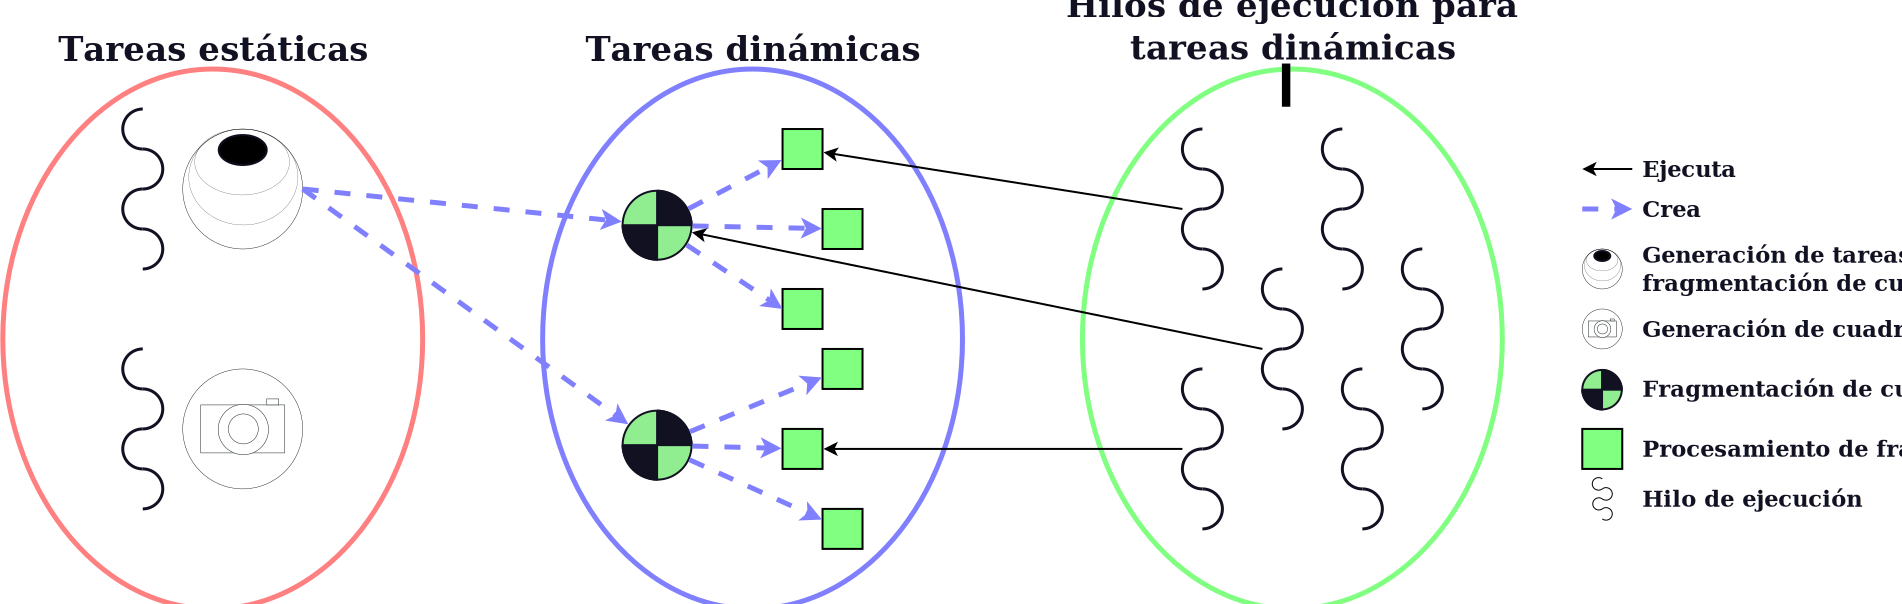
\includegraphics[width=\textwidth]{img/hilos.pdf}

	\caption{Asignación de tareas a los hilos de búsqueda.}

	\label{hilosFramework}

\end{figure}

\subsection{Fragmentación del conjunto de datos}

Para poder realizar el procesamiento paralelo, el conjunto de datos debe ser
fragmentado, en el caso del framework propuesto la división ser realizara en dos
niveles. Dado que el conjunto de datos es un vídeo, la primera fragmentación
consta de la separación en cuadros. Dado que cada cuadro es una captura del
ambiente completo en un instante de tiempo especifico distinto al de los demás
cuadros, se pueden procesar de forma independiente. La segunda fragmentación de
los datos se realiza dentro de cada cuadro. Dado que fragmentos de un mismo
cuadro contienen información distinta del ambiente sobre el mismo instante, los
fragmentos son dependientes entre si. Es por eso que se deben tener
consideraciones especiales para la división del cuadro.

Si el cuadro se divide en partes sin zonas solapadas puede suceder que los
parches de un robot se encuentren en fragmentos distintos. Esto es un problema,
ya que para encontrar los robots, el plugin de detección de robots debe detectar
todos los parches que lo identifican, por lo cual todos deben estar dentro del
mismo fragmento. Para asegurar esto, cada par de fragmentos adyacentes deben
compartir una zona igual al diámetro de un robot. En la figura
\ref{areaCompartida} se muestran los casos donde el área compartida es menor al
diámetro de un robot y donde el área compartida es del diámetro de un robot.

\begin{figure}[!h]

	\centering
	
\includegraphics[width=0.45\textwidth]{img/areaTooSmall.pdf}
	
\includegraphics[width=0.45\textwidth]{img/areaPerfect.pdf}

	\caption{Izquierda: si el área compartida es demasiado pequeña y el
	robot se encuentra entre dos fragmentos, puede que sus parches no sean
	completamente visibles desde ninguno de ellos. Derecha: si el área
	compartida es del ancho de los robots, entonces todos los parches son
	visibles completamente desde por lo menos un fragmento.}

	\label{areaCompartida}

\end{figure}

Dado que los fragmentos comparten una área en sus bordes, la suma del área de
los fragmentos es superior al área de la imagen original. Para reducir los
píxeles a procesar, se debe reducir la zona compartida. Como la zona compartida
tiene un ancho fijo (el diámetro de un robot), para encontrar el área compartida
mínima se debe minimizar el perímetro del fragmento.

Por la manera que las imágenes se representan comúnmente en una computadora y
por su simplicidad, se opto por trabajar con un teselado con rectángulos. En el
caso de estos, para minimizar su perímetro y maximizar su área, se debe procurar
que la relación entre su ancho y altura sea lo mas cercana a uno. También,
para balancear la carga uniformemente, todos los fragmentos serán de igual
tamaño\footnote{El tiempo de procesamiento de un fragmento depende no solo de su
área sino que es influido por los elementos encontrados por los plugins, por lo
cual fragmentos de igual tamaño pueden tener tiempos de procesamiento muy
distintos. Sin embargo, dado que no poseemos mas información antes del
procesamiento, consideramos que esta es la mejor heurística con la que
contamos}. Aquellos que se encuentren en los bordes inferior y derecho pueden
que sean mas chicos.

En la figura \ref{fragmentos} se muestran como se divide un cuadro de 800x600
píxeles con un área compartida de 50 píxeles en 1, 2, 5 y 8 fragmentos. Cuando
el número de fragmentos es un número primo, como en el caso de 5 fragmentos, el
cuadro se divide en franjas de igual ancho o altura que el cuadro original. Este
tipo de división produce fragmentos con perímetros mayores, produciendo grandes
áreas compartidas.

\begin{figure}[!h]

	
\includegraphics[width=0.5\textwidth]{img/fragmentos1.pdf}
	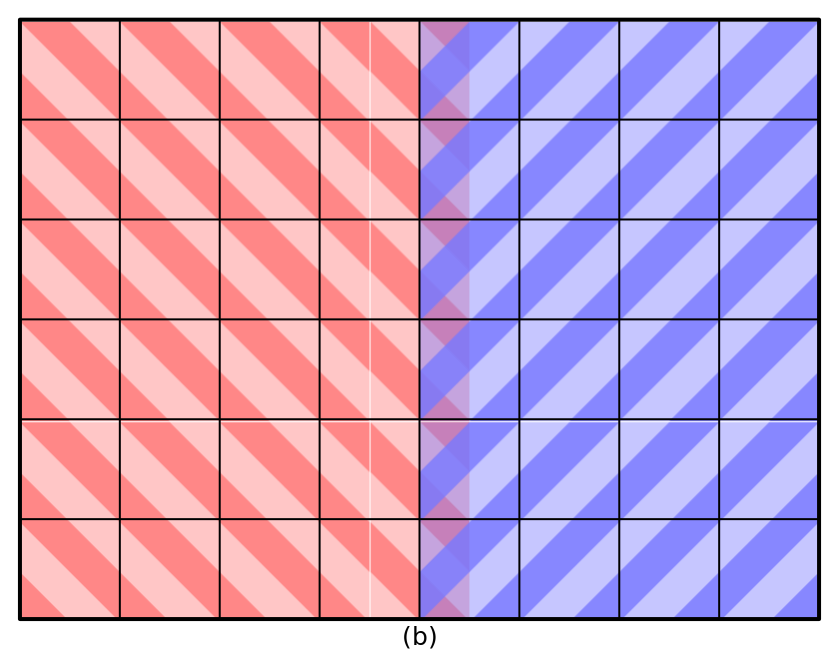
\includegraphics[width=0.5\textwidth]{img/fragmentos2.pdf}
	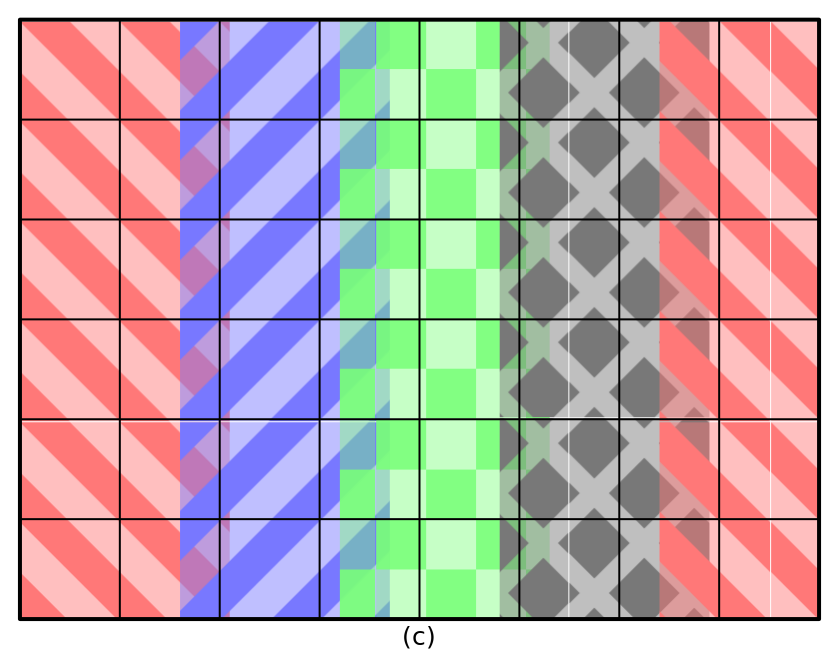
\includegraphics[width=0.5\textwidth]{img/fragmentos5.pdf}
	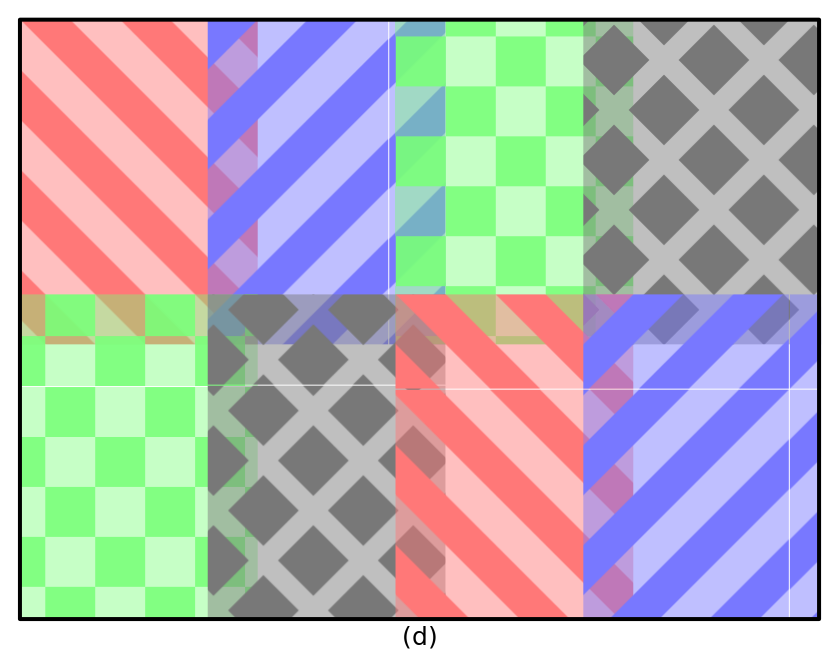
\includegraphics[width=0.5\textwidth]{img/fragmentos8.pdf}
	\caption{Resultado de dividir un cuadro de 800x600 píxeles con un área
	compartida de 50 píxeles en 1(a), 2(b), 5(c) y 8(d) fragmentos.}
	\label{fragmentos}

\end{figure}

\section{Implementación del framework}

El framework fue implementado en \emph{C++} con \emph{OpenMP} y está basado en
plugins para facilitar su modificación en un ambiente educativo.  La elección
del lenguaje se debe principalmente a su eficiencia y paradigma.  Dado que el
sistema debe procesar los cuadros en tiempos acotados, la eficiencia es crucial,
mientras que el paradigma orientado a objetos permite establecer fácilmente la
interfaz de los plugins. El uso de \emph{OpenMP} permite la creación y control
de hilos de ejecución y tareas de forma sencilla. Se utilizaron los plugins
implementados en \cite{torres2014}, modificándolos para permitir su uso en un
sistema paralelo.

\emph{OpenMP} es una API de bibliotecas y directivas al compilador para la
definición de paralelismo de alto nivel para sistemas de memoria compartida en
\emph{C}, \emph{C++} y \emph{Fortran}\cite{ompWeb}. La ventaja de \emph{OpenMP}
es que permite la creación de regiones paralelas, secciones criticas, tareas y
puntos de sincronización, simplemente marcando un bloque de código con unas
pocas directivas al compilador. \emph{OpenMP} originalmente implementaba solo el
modelo de \emph{fork and join}, pero a partir de la versión $3.0$ se agrego el
modelo de tareas explicitas\cite{openmp08}. Ambos modelos fueron utilizados para
la implementación del sistema.

El modelo de \emph{fork and join} fue propuesto por primera ves en
\cite{conway1963}. En este modelo, la ejecución del programa se ejecuta con un
solo hilo al comienzo de se ejecución y durante sus secciones secuenciales, al
hilo inicial se lo llama hilo principal. Cuando se encuentra una región de
trabajo compartido (o \emph{worksharing region}) de $N$ tareas, el hilo
principal crea $N-1$ nuevos hilos. Cada hilo (incluido el hilo principal)
ejecuta una de las $N$. Esta etapa es llamada \emph{fork}. El hilo principal no
continua la ejecución secuencial hasta que no han finalizado todas las tareas
paralelas. A esta sincronización se la llama \emph{join}. La figura \ref{conway}
muestra un ejemplo en el cual se crean dos tareas paralelas.

\begin{figure}[!h]

	\centering

	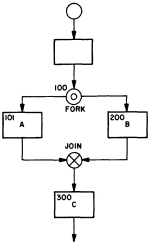
\includegraphics[width=0.25\textheight]{img/conway.pdf}

	\caption{Descripción original del modelo de \emph{fork and join}
	presentado por Melvin Conway en 1963\cite{conway1963}.}

	\label{conway}

\end{figure}

El modelo de \emph{fork and join} puede aplicarse tanto para paralelismo de
tareas como de datos. En el caso de \emph{OpenMP}, su uso para paralelismo de
datos se realiza comúnmente a través de la directiva \emph{parallel for},
mientras que la directivas \emph{parallel sections} y \emph{parallel section}
son utilizadas para el paralelismo de tareas.

Dado que la creación de hilos suele ser una operación costosa, la mayoría de las
implementaciones de \emph{OpenMP} suelen no destruir los hilos creados durante
el \emph{fork}, sino que se mantienen inactivos para ser reutilizados cuando se
encuentre otra región de trabajo compartido.

El segundo modelo implementado en \emph{OpenMP} a partir de la versión $3.0$ es
el de tareas. En este modelo cuando se encuentra una región de trabajo
compartido se crea un conjunto de $N$ hilos de ejecución, pero no se crean
tareas para esos hilos inmediatamente. Durante le ejecución de la región de
trabajo compartido, se crean tareas que son colocadas en una cola de ejecución.
Cuando un hilo de ejecución del conjunto esta libre se le asigna una tarea de la
cola de ejecución. Este modelo permite crear tareas de forma distribuida en el
tiempo, y la ejecución de mas tareas que la cantidad de hilos de ejecución
disponibles.

En la figura \ref{codigo} se muestra el fragmento de código (en pseudocódigo)
que ejecuta y crea las tareas principales del framework. En la función principal
(\emph{main}, linea 1 a 19) se crean las tareas de generación de cuadros (lineas
6 y 7) y generación de tareas de fragmentación de cuadros (lineas 8 a 10). El
control de la finalización del programa se controlara a través de una variable
compartida \emph{continuar}.

La tarea de generación de tareas de fragmentación de cuadros se implementa en la
función \emph{generaciónDeTareasDeFragmentaciónDeCuadros} (lineas 23 a 58). La
función comienza creando el pool de hilos de ejecución para tareas de búsqueda
(linea 25). También se crea un hilo adicional para la tarea de generación de
tareas fragmentación de cuadros. La tarea de generación de tareas de
fragmentación de cuadros implementa un espera ocupada sobre la cola de cuadros a
procesar para reducir el tiempo durante el cual los cuadros no se procesan aun
existiendo recursos libres. La tarea termina cuando la variable \emph{continuar}
es falsa.

Cuando hay hilos de ejecución libres y cuadros en la cola de cuadros, se toma un
cuadro de la cola de cuadros (lineas 29 a 32), se remueve un hilo del pool de
hilos de búsqueda para el cual se crea una tarea de fragmentación de cuadro con
una copia privada del puntero al cuadro (lineas 33 a 36).

Cada tarea de fragmentación de cuadro (lineas 37 a 53), comienza fragmentando el
cuadro. Por cada fragmento crea una tarea de procesamiento de fragmento,
asignándole a cada una un hilo del pool (lineas 40 a 43). Finalmente la tarea de
fragmentación de cuadro libera su hilo al finalizar.

Cada tarea de procesamiento de fragmento (lineas 44 a 52) procesa el fragmento
con cada pila (lineas 45 a 48). Cuando se termina de procesar el fragmento con
todas las pilas se borra el fragmento (linea 49) y se libera el hilo de
ejecución.

\begin{figure}[!h]

	\centering

	\includegraphics[width=0.5\textheight]{img/itemSwitch.pdf}

	\caption{Pseudo código del sistema}

	\label{codigo}

\end{figure}

\begin{figure}[!h]

	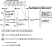
\includegraphics[width=\textwidth]{img/hilosytareas.pdf}

	\caption{Asignación de las tareas a los hilos de ejecución}

	\label{hilosytareas}

\end{figure}

Las clases del framework básico son las siguientes:

\begin{description}

	\item[Item:] Esta clase define un tipo genérico de los ítems que serán
		tratados por el sistema.

	\item[RingBuffer:] Este es el buffer donde se guardan los ítems
		generados mientras esperan ser procesados. El buffer guarda solo
		punteros a objetos de la clase \emph{Item} y no tiene mecanismos
		de control que permitan acceder la estructura desde múltiples
		hilos al mismo tiempo de forma segura. Cuando se solicita un
		ítem, se devuelve el puntero al mas antiguo o \textbf{NULL} en
		caso de que la estructura este vacía. Cuando se intenta agregar
		un nuevo ítem pero la estructura esta llena, se coloca este en
		el espacio del ítem mas viejo en la estructura y se retorna el
		puntero de este al llamador, delegándole su destrucción. La
		destrucción del ítem se delega al llamador por dos motivos. El
		primero es que el buffer desconoce el tipo real del ítem. La
		segunda razón es que para poder ser utilizado de forma segura,
		las llamadas a los métodos del buffer deben estar dentro de
		secciones criticas y realizar las eliminaciones dentro de estas
		podría ser muy lento.

	\item[Input:] Se trata de una clase que funciona como definición de la
		interfaz de las clases que generan los ítems. Sus métodos
		principales son \emph{run} y \emph{generate}. El método
		\emph{generate} debe ser re implementado por las clases hijas
		para generar el tipo de ítem especifico del sistema. El método
		\emph{run} es el encargado de generar los ítems llamando a
		\emph{generate} y colocarlos en el \emph{RingBuffer}. Este
		último método puede ser redefinido si la aplicación así lo
		requiere.

	\item[ItemSlicer:] Es la clase que define la interfaz de las clases
		encargadas de dividir los ítems. Se definen tres métodos. El
		primero es \emph{slice} que recibe como parámetro ítem y la
		cantidad de partes en la que este debe ser dividido y retorna un
		arreglo de ítems. El segundo método es \emph{resetItem} que
		recibe como parámetro una de las partes creadas por el método
		\emph{slice} luego de que fue procesada por una pila de plugins
		y la configura al estado para que el funcionamiento de la
		próxima pila no se vea interferido. El tercer método es
		\emph{delPart} que recibe como parámetro un fragmento de ítem y
		lo elimina.

	\item[Plugin:] Esta clase define una interfaz para los plugins que
		realizaran las distintas partes del procesamiento de la imagen.
		Solo se define el método \emph{process} que tiene como único
		parámetro un puntero a un objeto de la clase \emph{Item}.

	\item[PluginStack:] Esta es la clase que tomara el ítem y se encarga de
		entregarlo a cada uno de los plugins. Tiene solo dos métodos,
		\emph{addPlugin}, para agregar un plugin, y \emph{process} que
		tiene como parámetro un ítem, para procesarlo.

	\item[ItemSwitch:] Esta es la clase encargada de implementar la tarea de
		generación de tareas de fragmentación de cuadro. Para no crear
		mas tareas de las que puede procesar el sistema, solo se toma un
		cuadro de la cola de cuadros a procesar si hay hilos de búsqueda
		libres y no hay tareas ya creadas para asignarles. Cada tarea de
		fragmentación de cuadro divide el ítem utilizando
		\emph{ItemSlicer} y crea una nueva tarea de procesamiento de
		cuadros por cada fragmento.

\end{description}

\begin{figure}[h]

	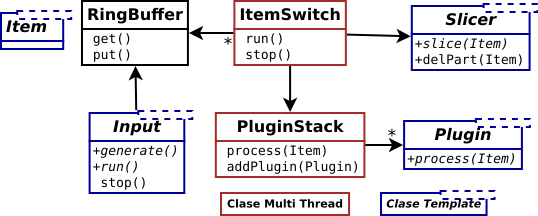
\includegraphics[width=\textwidth]{img/clasesFramework.pdf}

	\caption{Diagrama de clases Framework base.}

\end{figure}

Existen dos parámetros ajustables. El primero es la cantidad de hilos que
ejecutaran las tareas de búsqueda. El segundo parámetro es la cantidad de partes
en las cuales se dividirá el cuadro.

Para adaptar el framework para utilizarlo como un sistema de visión por
computadora para el fútbol de robots se incorporaron las siguientes clases, las
cuales fueron tomadas y modificadas del sistema de visión presentado en
\cite{torres2014}:

\begin{description}

	\item[Frame:] Subclase de \emph{Item}. Contiene una imagen que
		representa un cuadro y una estructura auxiliar que contiene la
		información necesaria para el funcionamiento de los plugins.

	\item[CaptureFromFile:] Subclase de \emph{Input}. Es la clase encargada
		de crear el flujo de objetos \emph{Frame}, tomando cada cuadro
		desde un archivo de vídeo. También debe respetar la taza de
		cuadros por segundo del vídeo.

	\item[FastCaptureFromFile:] Subclase de \emph{Input}. Muy similar a
		\emph{CaptureFromFile}, con las diferencias de que carga los
		cuadros a memoria antes de que comience el sistema a capturar
		los cuadros (para evitar los retardos de la lectura de disco y
		decodificación), y que tiene dos modos de controlar la
		frecuencia de la generación de los cuadros. Se puede adelantar
		la creación de cuadros si la cola de cuadros a procesar esta
		vacía, o fijar la frecuencia de su creación a un valor
		especifico. Esta clase es útil para comprobar la capacidad
		máxima del sistema, ya que permite simular una cámara con la
		velocidad de captura que se desee, y los distintos modos
		permiten testear la carga máxima en cuadros por segundo
		soportada por el sistema, así como los tiempos de espera bajo
		una cantidad de cuadros por segundo especifica.

	\item[FrameSlicer:] Subclase de \emph{ItemSlicer}. En este caso lo que
		se divide es la imagen del cuadro. Cada sub cuadro tendrá un
		solapamiento con los adyacente ya que se debe evitar que un
		robots o la pelota no este totalmente contenido dentro de por lo
		menos un sub cuadro. Para minimizar el área solapada, las
		particiones se realizan de manera tal que se minimice el
		perímetro pero ocupen la mayor área posible. Para lograr esto se
		busca la partición que haga que la relación entre el alto y el
		ancho sea lo mas cercana a uno.

	\item[Subclases de \emph{Plugin}:] \emph{PluginBlur},
		\emph{PluginColorConversions}, \emph{PluginColorSegmentation},
		\emph{PluginDetectBalls}, \emph{PluginFindBlobs},
		\emph{PluginFindSecondariesBlobs}, \emph{PluginMorphology} y
		\emph{PluginNetworking}.

	\item[Clases auxiliares:] \emph{ball}, \emph{colorspace},
		\emph{datastruct}, \emph{homography}, \emph{marker},
		\emph{pattern}, \emph{pattern\_matching},
		\emph{practicalsocket}, \emph{segmentation}, \emph{team},
		\emph{timer}.

\end{description}

\begin{figure}[h]

	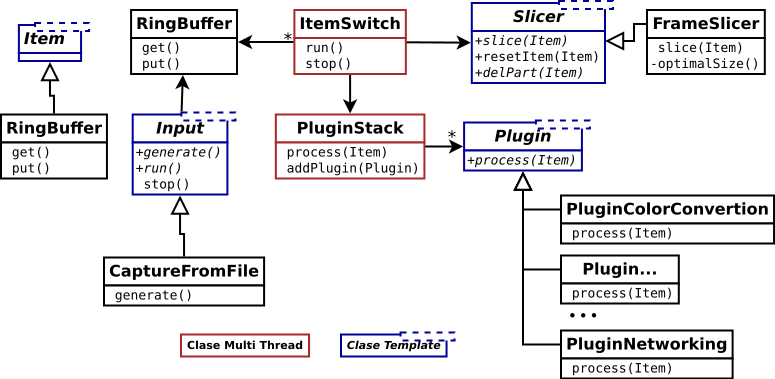
\includegraphics[width=\textwidth]{img/clasesFrameworkRobots.pdf}

	\caption{Diagrama de clases del sistema sistema de visión para el fútbol
	de robots.}

\end{figure}

Conceptualmente, la implementación para fútbol de robots tiene dos pilas, una
para búsqueda de robots y la otra para búsqueda de la pelota. Sin embargo, ambas
pilas utilizan los mismos plugins con la misma configuración para la etapa de
pre procesamiento de la imagen, ademas, los plugins que no tienen en común solo
modifican datos propios de cada pila. Esto permite que ambas pilas puedan ser
unidas en una sola, lo que trae como ventaja que la etapa de pre procesamiento
se realice solo una ves por fragmento.
